\section{Sprint 2}

\subsection{Sprint Planning}

Objetivo da Sprint: Produzir a seção de Introdução da proposta de TCC e descrever claramente o problema e objetivos do trabalho.

\begin{table}[htbp]
  \centering
  \caption{Sprint backlog e tarefas — Sprint 2}
  \label{tab:sprint2}
  \begin{tabular}{ccc}
    \toprule
    Tarefa & Descrição & Estimativa (pessoas·hora) \\
    \midrule
    US-02A & Esboçar tópicos da Introdução & 2 \\
    US-02B & Redigir rascunho da Introdução & 4 \\
    US-02C & Revisar e incluir referências & 1 \\
    US-03A & Descrever problema e objetivos & 5 \\
    US-03B & Revisar clareza dos objetivos & 3 \\
    \bottomrule
  \end{tabular}
  \fonte{Elaboração própria.}
\end{table}

\vspace{0.5em}
\noindent\textbf{Capacidade utilizada:} 15 pessoas·hora (100\% da velocidade da equipe)

\subsection{Quadro Kanban}

Histórico da evolução do quadro Kanban no início e ao final de cada Sprint.

\begin{figure}[htbp]
  \centering
  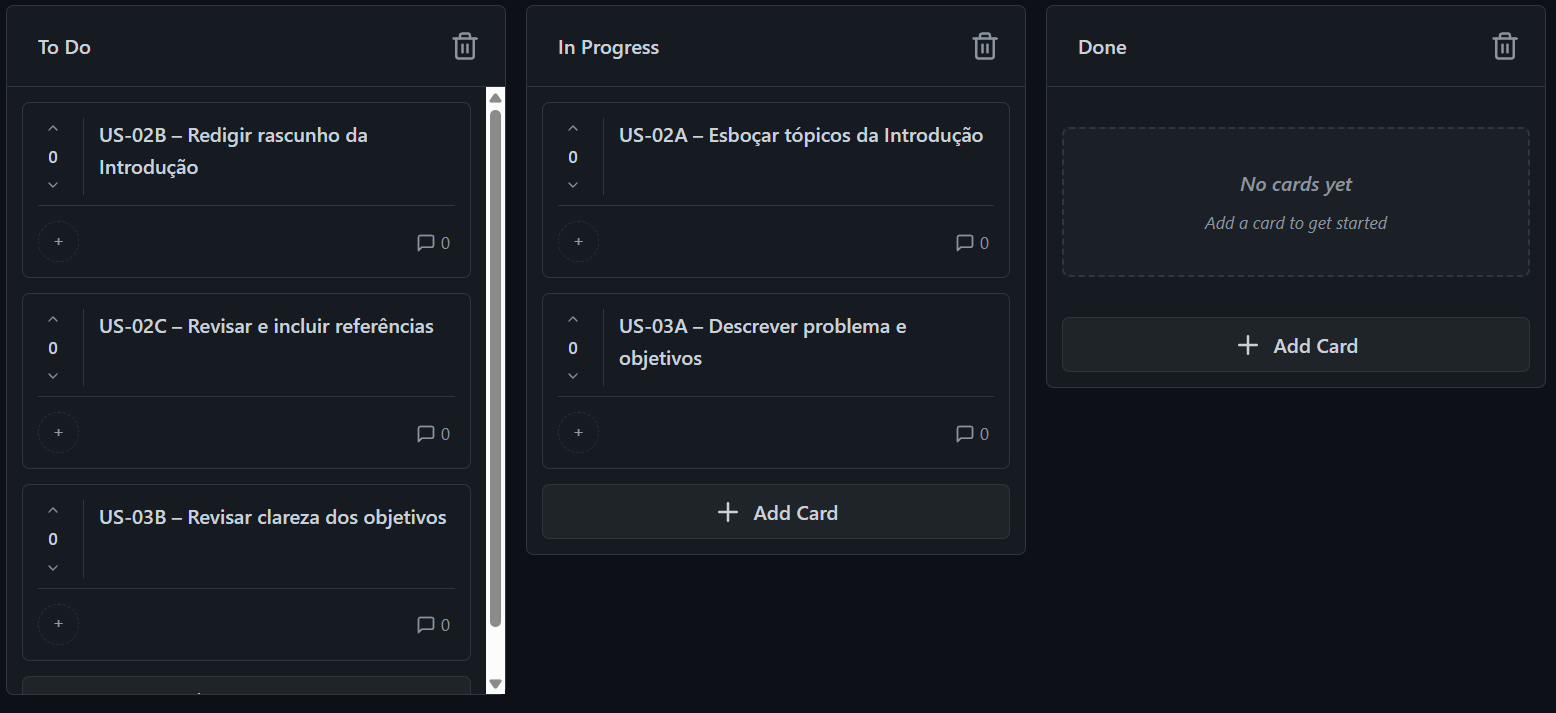
\includegraphics[width=0.8\linewidth]{pictures/kanban_sprint2_inicio.png}
  \caption{Visão geral do Quadro Kanban no início da Sprint 2}
\end{figure}

\begin{figure}[htbp]
  \centering
  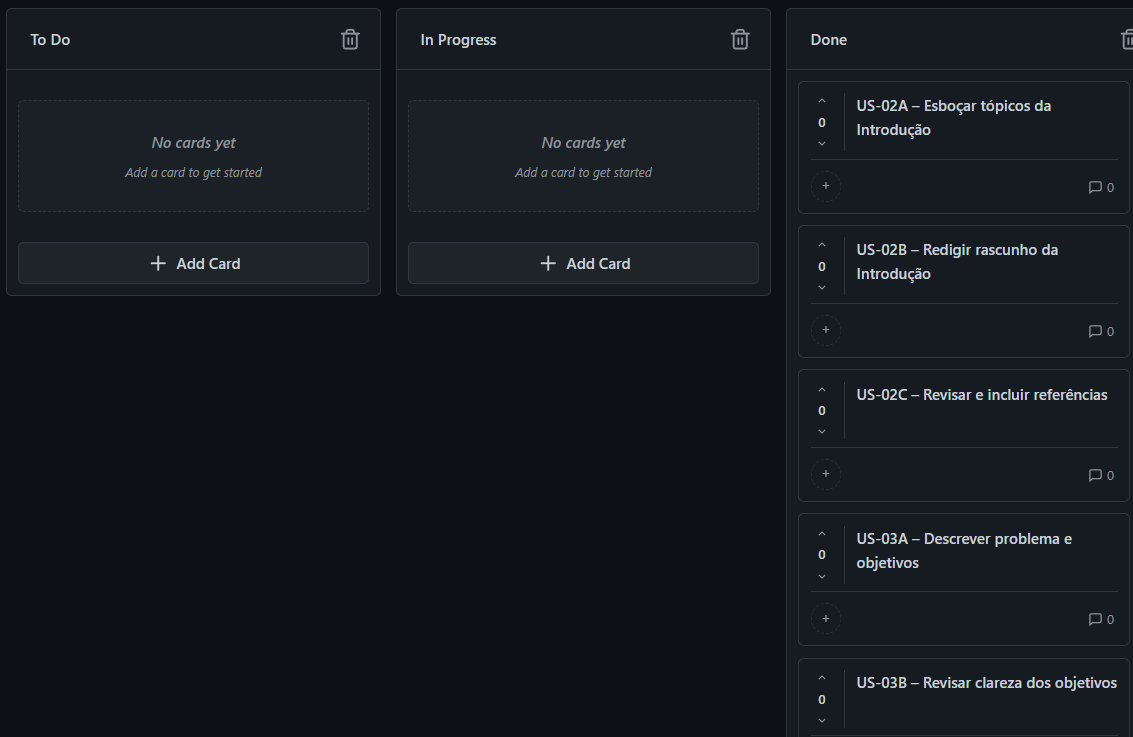
\includegraphics[width=0.8\linewidth]{pictures/kanban_sprint2_final.png}
  \caption{Visão geral do Quadro Kanban ao final da Sprint 2}
\end{figure}


\subsection{Reuniões de Acompanhamento}

Daily 3 (\textless Data\textgreater): Não houve.

\begin{figure}[htbp]
  \centering
  \includegraphics[width=0.6\linewidth]{pictures/daily3.png}
  \caption{Evidência da Daily 3}
\end{figure}

Daily 4 (21/06/2025): Todas as tarefas foram concluídas.

\begin{figure}[htbp]
  \centering
  
\includegraphics[width=0.6\linewidth]{pictures/daily4.png}
  \caption{Evidência da Daily 4}
\end{figure}

\begin{figure}[htbp]
  \centering
  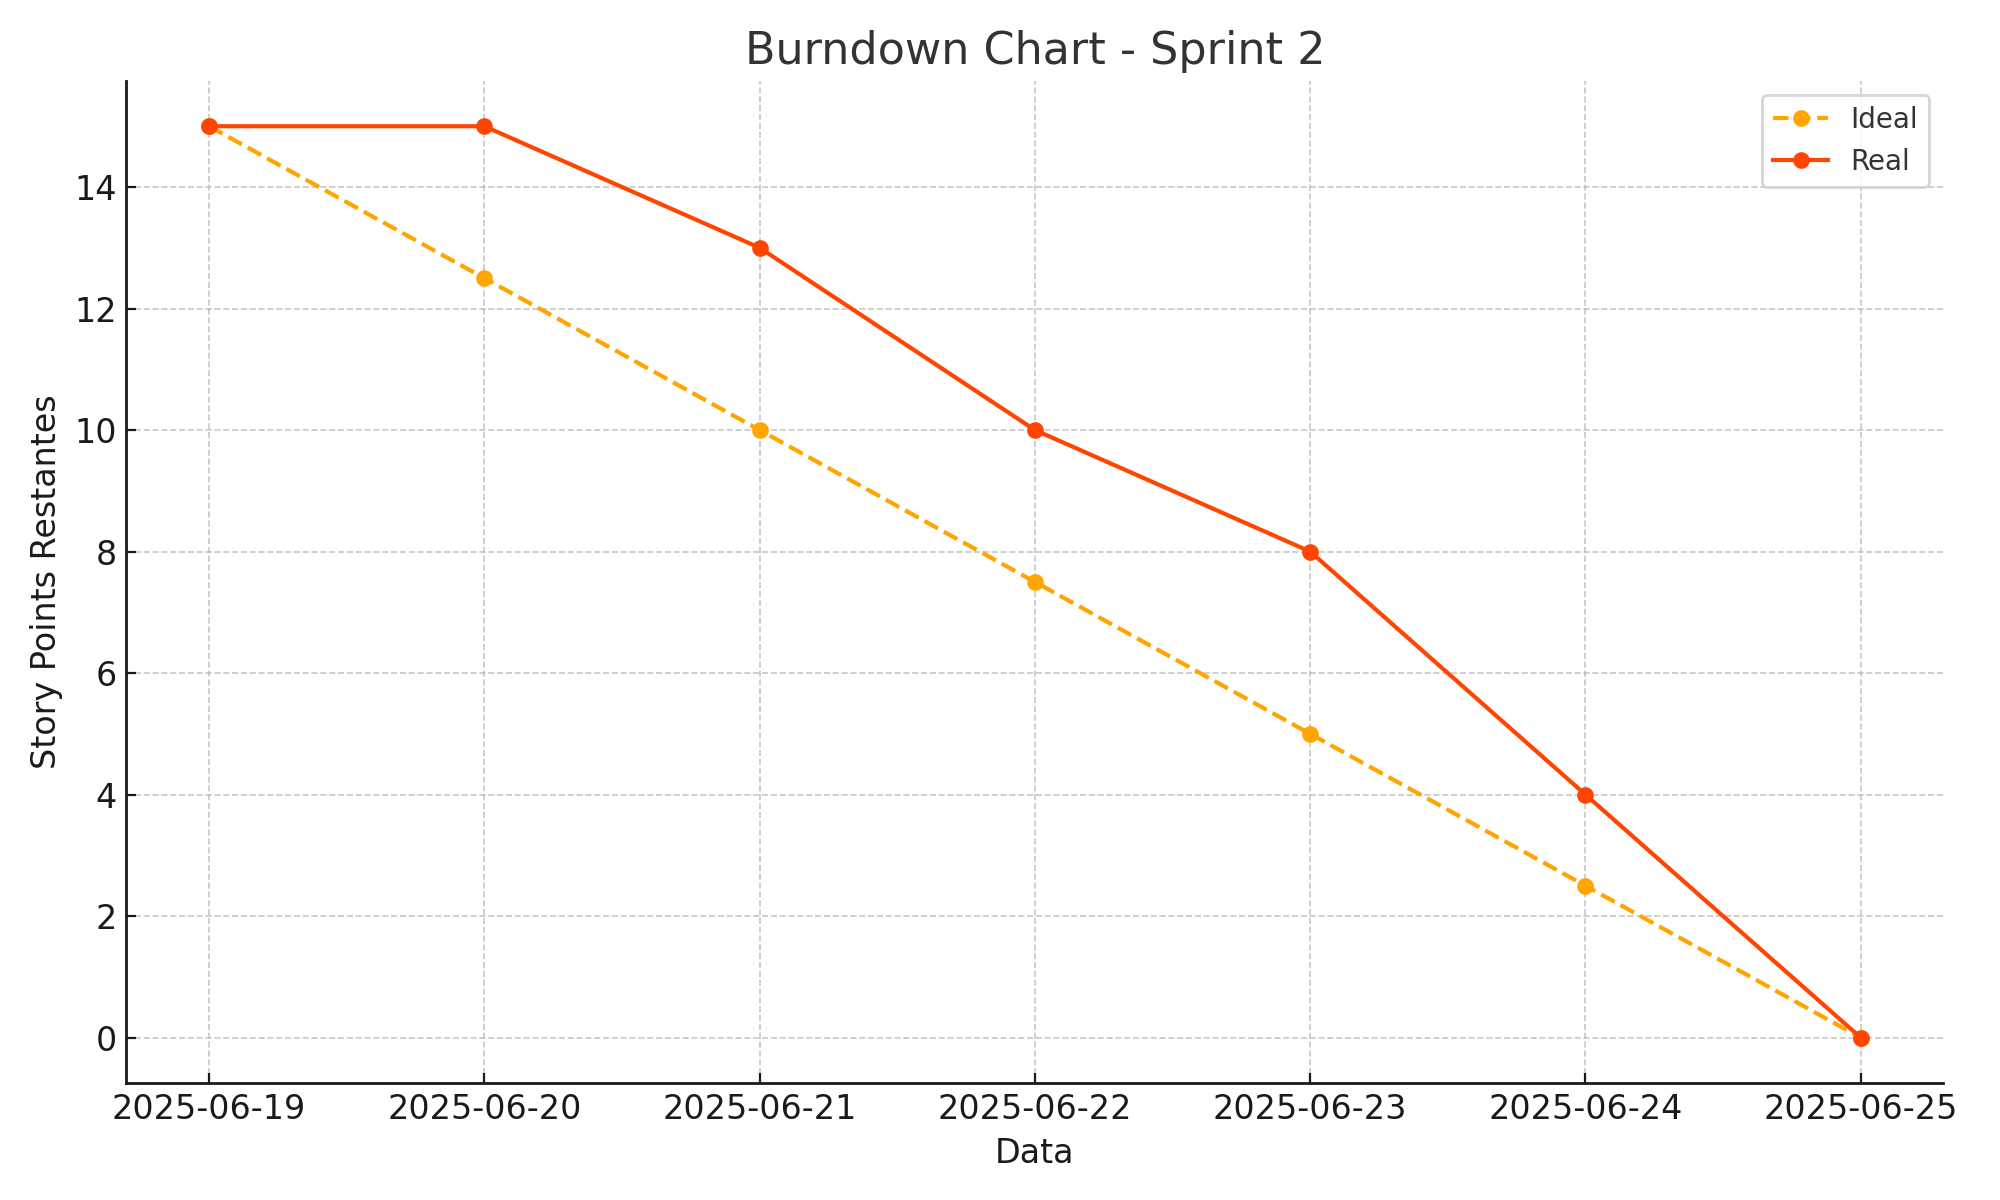
\includegraphics[width=0.7\linewidth]{pictures/burndown_sprint2.png}
  \caption{Burndown — Sprint 2}
\end{figure}



\subsection{Resultados das Sprints}

A Sprint 2 focou na redação da Introdução e na definição clara dos objetivos do trabalho. Apesar do escopo enxuto, a equipe conseguiu avançar de forma eficiente, finalizando a maior parte das tarefas planejadas. Identificou-se, no entanto, que seria possível assumir uma carga de trabalho maior.

\begin{table}[htbp]
  \centering
  \caption{Resultados — Sprint 2}
  \label{tab:resultSprint2}
  \begin{tabular}{lll}
    \toprule
    ID & Tarefa & Status \\
    \midrule
    US-02A & Esboçar tópicos da Introdução & Concluída \\
    US-02B & Redigir rascunho da Introdução & Concluída \\
    US-02C & Revisar e incluir referências & Concluída \\
    US-03A & Descrever problema e objetivos & Concluída \\
    US-03B & Revisar clareza dos objetivos & Concluída \\
    \bottomrule
  \end{tabular}
  \fonte{Elaboração própria.}
\end{table}

\vspace{1em}
\noindent\textbf{Resumo da Sprint:}
\begin{itemize}[noitemsep]
  \item Tarefas previstas: 5
  \item Concluídas: 5
\end{itemize}

\noindent\textbf{Aprendizados e observações:}
\begin{itemize}
  \item O escopo da sprint foi subestimado — poderia ter mais tasks.
\end{itemize}

% Evidências gráficas
\begin{figure}[htbp]
  \centering
  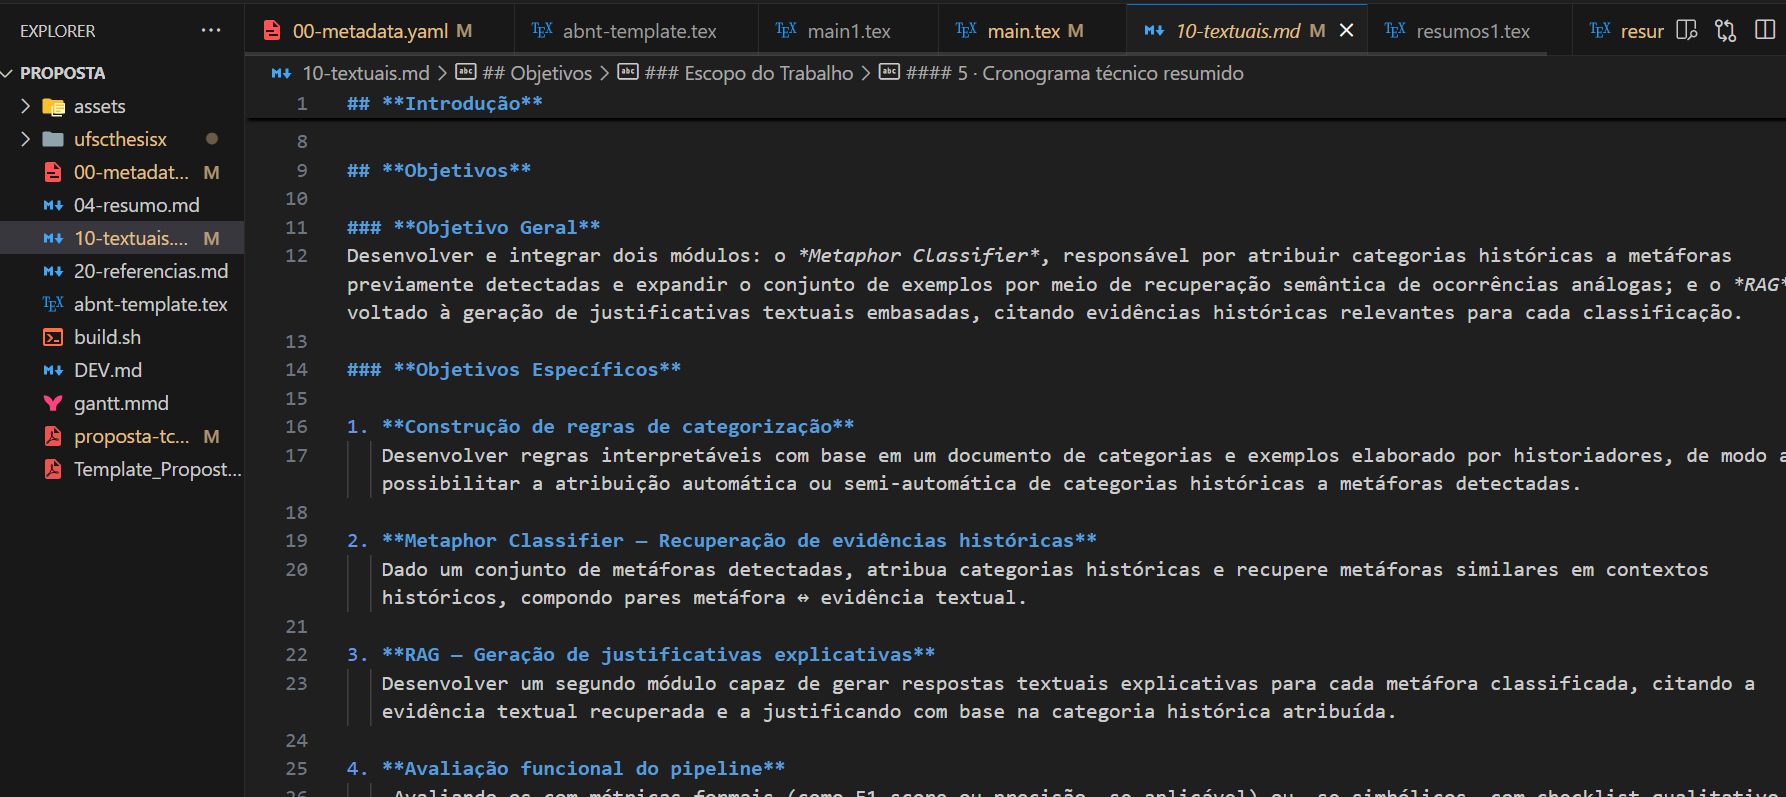
\includegraphics[width=0.6\linewidth]{pictures/intro_topicos.png}
  \caption{Evidência da tarefa US-02A}
\end{figure}

\begin{figure}[htbp]
  \centering
  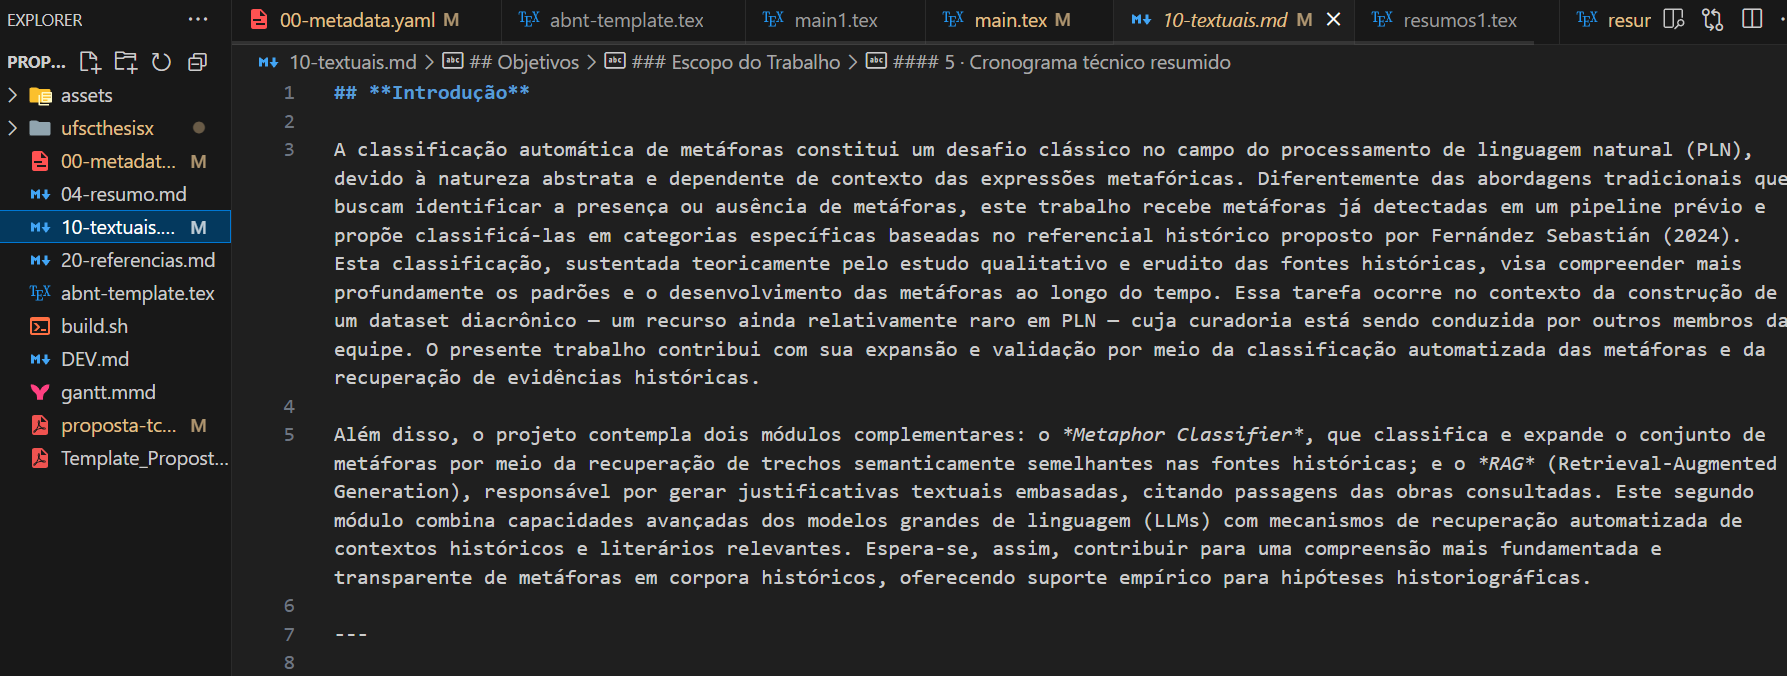
\includegraphics[width=0.6\linewidth]{pictures/intro_rascunho.png}
  \caption{Evidência da tarefa US-02B}
\end{figure}

\begin{figure}[htbp]
  \centering
  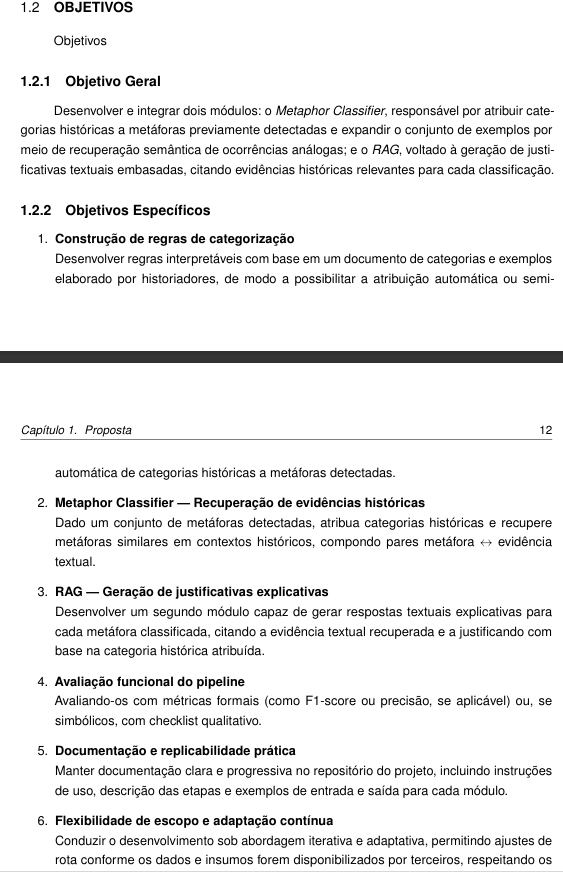
\includegraphics[width=0.6\linewidth]{pictures/problema_objetivos.png}
  \caption{Evidência da tarefa US-03A}
\end{figure}



\subsection{Retrospectivas}

\begin{itemize}
  \item \textbf{Pontos de atenção}:
  \begin{itemize}
    \item Houve apenas uma daily.
    \item O escopo da sprint foi subdimensionado: todas as tarefas foram concluídas rapidamente, sugerindo que seria possível incluir mais atividades.
  \end{itemize}

  \item \textbf{O que pode ser melhorado}:
  \begin{itemize}
    \item Garantir acompanhamento contínuo (respeitar as dailies).
    \item Refinar o planejamento de sprint com base na capacidade real do grupo, prevendo mais tarefas quando possível.
  \end{itemize}

  \item \textbf{O que manter/continuar}:
  \begin{itemize}
    \item Boa execução e comprometimento da equipe com as entregas.
    \item Clareza nos objetivos da sprint facilitou o foco e a conclusão eficiente das tarefas.
  \end{itemize}
\end{itemize}

\vspace{1em}
\noindent\textbf{Burndown Chart:}

\begin{center}
  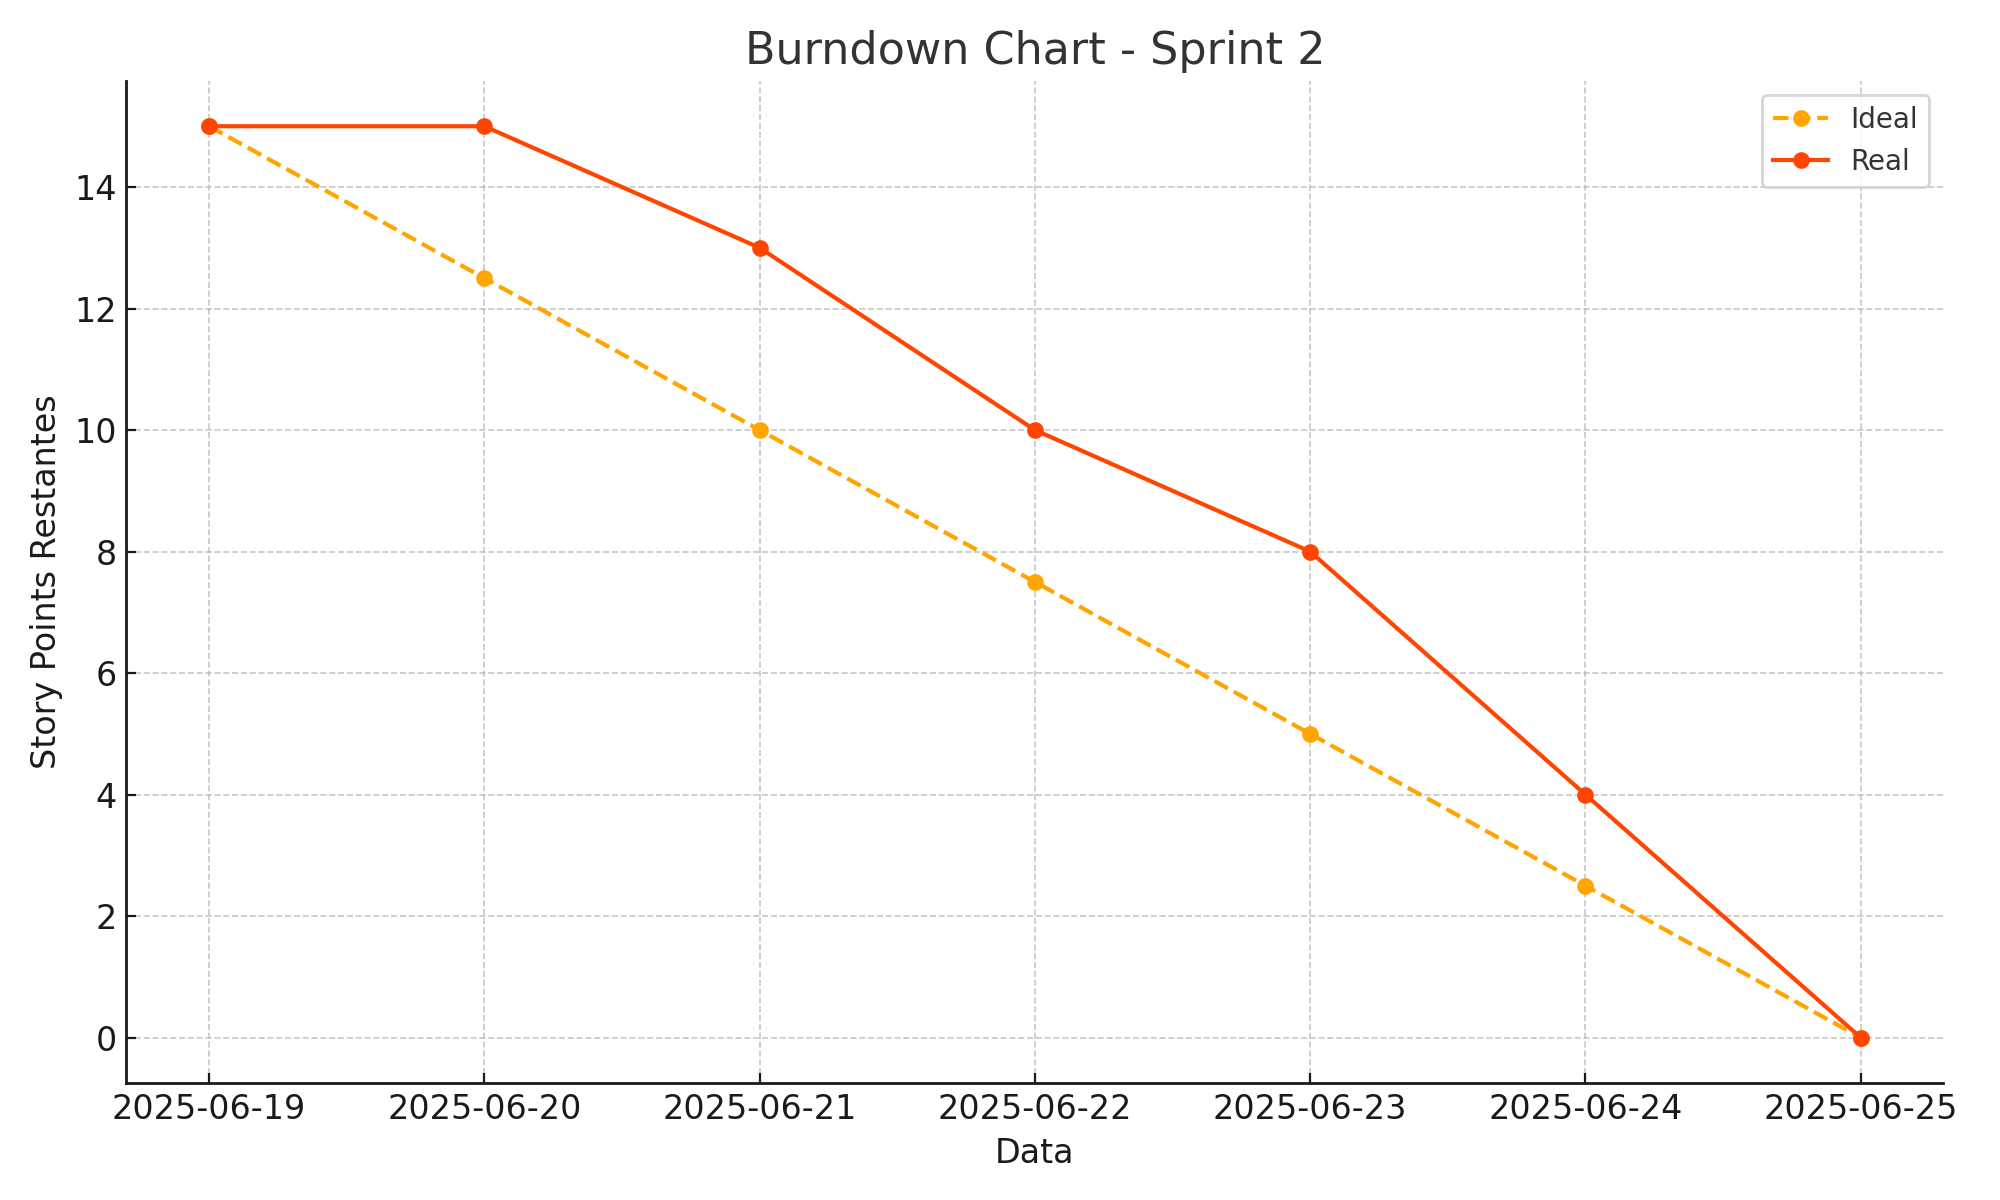
\includegraphics[width=0.8\textwidth]{pictures/burndown_sprint2.png}
\end{center}
